\documentclass[bigger]{beamer}
\usepackage[spanish, es-tabla]{babel}
\usepackage[utf8]{inputenc}
\usepackage[T1]{fontenc}
\usepackage{xcolor}
\usepackage{amsmath}
\usepackage{xcolor}
\usepackage{enumitem}
\usepackage{subfig}
\usepackage{datetime}
\usepackage{multicol}
\usepackage[underline=false, rounded corners=false]{pgf-umlsd}
\usepackage{eforms}
% Tablas
\usepackage{tabularx}
\usepackage{booktabs}
\usepackage{array}
\newcolumntype{L}[1]{>{\raggedright\let\newline\\\arraybackslash\hspace{0pt}}m{#1}}
\newcolumntype{C}[1]{>{\centering\let\newline\\\arraybackslash\hspace{0pt}}m{#1}}
\newcolumntype{R}[1]{>{\raggedleft\let\newline\\\arraybackslash\hspace{0pt}}m{#1}}

% Figuras
\usepackage{standalone}
\usepackage{tikz}
\usetikzlibrary{
    automata, 
    positioning,
    calc, 
    arrows, 
    shapes.geometric,  
    shapes.symbols,
    backgrounds
}

% Tick y cruz
\usepackage{pifont}
\newcommand{\cmark}{\ding{51}}%
\newcommand{\xmark}{\ding{55}}%

\usepackage{graphicx}
\newdate{fecha}{14}{7}{2022}

\decimalpoint

% Definición colores
\definecolor{verdedato}{RGB}{78,173,50}
\definecolor{rojodato}{RGB}{234,51,35}
\definecolor{azuldato}{RGB}{0,0,200}

\definecolor{codegreen}{RGB}{184,215,163}
\definecolor{codegray}{rgb}{0.5,0.5,0.5}
\definecolor{codepurple}{rgb}{0.58,0,0.82}
\definecolor{backcolour}{rgb}{0.95,0.95,0.92}

\definecolor{azuldiagrama}{RGB}{93,160,242}
\definecolor{verdediagrama}{RGB}{124,244,111}
\definecolor{rojodiagrama}{RGB}{204,73,53}
\definecolor{naranjadiagrama}{RGB}{209,139,69}
\definecolor{blancodiagrama}{RGB}{237,247,211}

\definecolor{azulclasificador}{RGB}{181,199,230}
\definecolor{verdeclasificador}{RGB}{197,224,181}
\definecolor{rojoclasificador}{RGB}{248,204,175}

\definecolor{rojoUMU}{RGB}{189,42,51}
\newcommand{\rojoUMU}[1]{\textcolor{rojoUMU}{#1}}

\renewcommand{\labelitemi}{$\blacktriangleright$}
\renewcommand{\labelitemii}{$\textcolor{rojoUMU}{\vartriangleright}$}

%%%%%%% Title Page %%%%%%%
\title{Identificación de dispositivos IoT a través de huellas hardware}
%\subtitle{Subtítulo de la presentación, más largo que el título, pero no mucho}
\date{\displaydate{fecha}}
\author{Sergio Marín Sánchez
 }
%\institute{Universidad de Murcia \\ Facultad de Informática}

%Title color
\setbeamercolor*{title}{fg=white}   
%Title size, font family, font weight
\setbeamerfont{title}{size=\LARGE,series=\bfseries,parent=structure,family=\rmfamily} 

%Subtitle color
\setbeamercolor*{subtitle}{fg=white}  
%Subtitle size, font family, font weight
\setbeamerfont{subtitle}{size=\normalsize,series=\bfseries,parent=structure,family=\rmfamily} 

%Date color
\setbeamercolor*{date}{fg=white}   

%Author color
\setbeamercolor*{author}{fg=white}  

%Institution color
\setbeamercolor*{institute}{fg=white}  

%Section colors
\setbeamercolor*{section in toc}{fg=white}  
\setbeamercolor*{subsection in toc}{fg=white} 

%Table of contents font size
%\setbeamerfont{section in toc}{size=\scriptsize}

%Table of contents style
\setbeamertemplate{section in toc}[circle]
\setbeamercolor{section number projected}{bg=black}

%%%%%%%%%%%%%%%%%%%%%%%%%%%%

%%%%%%% Global Settings %%%%%%%

%Headers color
\setbeamercolor{frametitle}{fg=white}
%Headers, font family, font weight
\setbeamerfont{frametitle}{size=\Large,series=\bfseries,parent=structure,family=\rmfamily}

%Subheaders color
\setbeamercolor{framesubtitle}{fg=white}
%Subheaders, font family, font weight
\setbeamerfont{framesubtitle}{size=\footnotesize,series=\bfseries,parent=structure,family=\rmfamily}

%Caption color
\setbeamercolor{caption name}{fg=rojoUMU}

%Items color
\setbeamercolor{itemize item}{fg=black}

%Background image
\usebackgroundtemplate{\includegraphics[width=\paperwidth,height=\paperheight]{/Users/serms1999/Pictures/Fondo3.png}}

%%%%%%%%%%%%%%%%%%%%%%%%%%%%

%%%%%%% Math Settings %%%%%%%

\DeclareMathOperator*{\minimize}{min}
%etc.

%%%%%%%%%%%%%%%%%%%%%%%%%%%%

\makeatletter
\tikzset{
    database top segment style/.style={draw},
    database middle segment style/.style={draw},
    database bottom segment style/.style={draw},
    database/.style={
        path picture={
            \path [database bottom segment style]
                (-\db@r,-0.5*\db@sh) 
                -- ++(0,-1*\db@sh) 
                arc [start angle=180, end angle=360,
                    x radius=\db@r, y radius=\db@ar*\db@r]
                -- ++(0,1*\db@sh)
                arc [start angle=360, end angle=180,
                    x radius=\db@r, y radius=\db@ar*\db@r];
            \path [database middle segment style]
                (-\db@r,0.5*\db@sh) 
                -- ++(0,-1*\db@sh) 
                arc [start angle=180, end angle=360,
                    x radius=\db@r, y radius=\db@ar*\db@r]
                -- ++(0,1*\db@sh)
                arc [start angle=360, end angle=180,
                    x radius=\db@r, y radius=\db@ar*\db@r];
            \path [database top segment style]
                (-\db@r,1.5*\db@sh) 
                -- ++(0,-1*\db@sh) 
                arc [start angle=180, end angle=360,
                    x radius=\db@r, y radius=\db@ar*\db@r]
                -- ++(0,1*\db@sh)
                arc [start angle=360, end angle=180,
                    x radius=\db@r, y radius=\db@ar*\db@r];
            \path [database top segment style]
                (0, 1.5*\db@sh) circle [x radius=\db@r, y radius=\db@ar*\db@r];
        },
        minimum width=2*\db@r + \pgflinewidth,
        minimum height=3*\db@sh + 2*\db@ar*\db@r + \pgflinewidth,
    },
    database segment height/.store in=\db@sh,
    database radius/.store in=\db@r,
    database aspect ratio/.store in=\db@ar,
    database segment height=0.1cm,
    database radius=0.25cm,
    database aspect ratio=0.35,
    database top segment/.style={
        database top segment style/.append style={#1}},
    database middle segment/.style={
        database middle segment style/.append style={#1}},
    database bottom segment/.style={
        database bottom segment style/.append style={#1}}
}
\makeatother

\tikzset{
    ->,  % makes the edges directed
    >=stealth', % makes the arrow heads bold
    every state/.style={thick, fill=gray!10}, % sets the properties for each ’state’ node
    initial text=$ $, % sets the text that appears on the start arrow
}


\includeonly{
    Introduccion,
    EstadoArte,
    DisenoImplementacion,
    ExperimentosResultados,
    Conclusiones
}

\begin{document}

%Title Slide
{\usebackgroundtemplate{\includegraphics[width=\paperwidth]{/Users/serms1999/Pictures/Fondo1.png}} %Title Background
\begin{frame}
\rmfamily %Title Font
\color{white} %Title Color & Weight
\vspace{2.3cm}
\begin{center}
    \bfseries
    \Large
    Identificación de dispositivos IoT \\
    a través de huellas hardware
\end{center}
% Author and supervisor
\begin{minipage}{0.5\textwidth}
\begin{flushleft}
\emph{Autor:}\\
Sergio \textsc{Marín Sánchez}\\
\end{flushleft}
\end{minipage}
\begin{minipage}{0.45\textwidth}
\begin{flushright}
\emph{Tutores:} \\
Gregorio \textsc{Martínez Pérez}\\
Pedro Miguel \textsc{Sánchez Sánchez}\\
\end{flushright}
\end{minipage}
\end{frame}
}

\newcommand{\RN}[1]{%
  \ensuremath{\textup{\uppercase\expandafter{\romannumeral#1}}}%
}

%Contents Slide
{\usebackgroundtemplate{\includegraphics[width=\paperwidth]{/Users/serms1999/Pictures/Fondo2.png}} %Contents Background
\begin{frame}
\frametitle{Índice} %Contents Title
\rmfamily %Contents Font
\color{white}
\tableofcontents[hideallsubsections]
\end{frame}
}

%!TEX root = TFG.tex

\chapter{Introducción} \label{chap:intro}

\section{Contexto}

En los últimos años el número de dispositivos conectados a internet se ha incrementado en gran medida \cite{84Billio53:online}. Esto se debe al uso de smartphones, tablets y demás dispositivos que requieren de conexión a internet para llevar a cabo la mayoría (o la totalidad) de tareas para las que han sido diseñados.

Cada dispositivo conectado a internet tiene asociados varios identificadores, como la dirección IP y la dirección MAC. Estos identificadores deberían servir para identificar unívocamente a un dispositivo, pero en la práctica no se da esta situación. Las direcciones IP pueden cambiar automáticamente debido al direccionamiento IP dinámico (mediante servidores DHCP), pero también pueden ser modificadas por las propias personas. 

Estas modificaciones pueden ser por temas únicamente de privacidad, pero en muchas ocasiones están relacionadas con la ciberdelincuencia. Los delicuentes pueden intentar falsificar sus identificadores con el objetivo de que las personas, buscando conectarse a un servicio legítimo, acaben conectándose a sus equipos.

Los fines de esto son, por ejemplo, introducir virus en sus equipos, para realizar ataques DDoS (ataques de denegación de servicio distribuidos) mediante miles de equipos infectados, para cifrar los datos de dicho equipo (ataque de ransomware), para realizar ataques de phishing, enviando páginas visualmente idénticas a las que consulte el equipo, pero los datos sensibles de los formularios (contraseñas) pasen a disposición del atacante. Otro fin posible es el mero espionaje de los datos.

\section{Motivación}

Es en este punto en el que se requieren técnicas de comunicación seguras entre los dispositivos. Desde el punto de vista de las redes existen protocolos de comunicación segura como SSL, TLS, IPsec, etc. Pero estos dispositivos son inútiles si el equipo se quiere conectar voluntariamente al equipo atacante (esto debido al engaño que se ha comentado anteriormente).

Por estos motivos, existe la pregunta sobre cómo podemos saber a qué equipos nos estamos conectando, o qué diferencia a un dispositivo de otro en internet si ambos presentan los mismos identificadores.

Una respuesta a estas preguntas es que los dispositivos aunque presenten el mismo hardware, tengan los mismos identificadores y ejecuten el mismo software, nunca serán exactamente iguales. Esto es debido a que en el proceso de fabricación de los dispositivos siempre habrá diferencias (por pequeñas que sean) que harán que los dispositivos sean distinguibles entre sí, por ejemplo, un dispositivo ejecuta una función en \SI{1.2}{\nano\second} y otro en \SI{1.4}{\nano\second}. Las diferencias son mínimas pero existen.

En el panorama actual del big data y el machine learning podemos explotar estas diferencias de tal forma que se generen huellas de cada dispositivo y con ello saber si realmente nos estamos conectando con el dispositivo adecuado o no.

En este marco de trabajo es en el que se centra este proyecto. Se busca crear un sistema que partiendo de un reloj exacto, compare las desviaciones de los relojes de los distintos dispositivos y con ello cree una huella estadística del comportamiento de cada uno. Posteriormente se automatizará el proceso de analizar esos valores estadísticos mediante un modelo de machine learning.

\section{Objetivos}

Para lograr nuestro objetivo final de identificar dispositivos idénticos de forma automática, podemos establecer diversas metas intermedias.

\begin{itemize}
    \item \textbf{Objetivo 1}. Presentar la arquitectura IoT, así como sus diversas aplicaciones.
    \item \textbf{Objetivo 2}. Presentar distintas soluciones dentro del campo del Machine Learning que pueden ser aplicadas a nuestro problema.
    \item \textbf{Objetivo 3}. Analizar las distintas formas de obtener una marca de tiempo, con suficiente precisión, de un dispositivo.
    \item \textbf{Objetivo 4}. Generar un dataset con las distintas desviaciones de reloj de los dispositivos bajo análisis.
    \item \textbf{Objetivo 5}. Analizar estadísticamente las diferencias entre los distintos relojes de los dispositivos, con el fin de ver si son estadísticamente diferenciables.
    \item \textbf{Objetivo 6}. Generar un nuevo dataset con distintas variables estadísticas de las desviaciones previas.
    \item \textbf{Objetivo 7}. Dividir el nuevo dataset en conjuntos de entrenamiento y test para los modelos de Machine Learning, de forma que no se pierdan las características del mismo.
    \item \textbf{Objetivo 8}. Evaluar distintos algoritmos de Machine Learning para la tarea de distinguir entre los dispositivos.
    \item \textbf{Objetivo 9}. Describir las futuras vías de investigación de trabajos similares a este.
\end{itemize}

\section{Estructura del documento}

Este documento está compuesto en primer lugar por un resumen, tanto en español como en inglés (de forma extendida), seguidos de 6 capítulos.

\begin{itemize}
    \item \textbf{Capítulo \ref{chap:intro}}. Es el capítulo actual, donde se presentan el contexto, la motivación y los objetivos del trabajo.
    \item \textbf{Capítulo \ref{chap:art}}. En este capítulo se realiza una presentación de la arquitectura IoT y sus aplicaciones, así como, una presentación del Machine Learning y algunos de sus algoritmos.
    \item \textbf{Capítulo \ref{chap:meto}}. 
    \item \textbf{Capítulo \ref{chap:diseno}}. En este capítulo se hablará de nuestra propuesta para abordar este problema. Se obtendrán varios dataset y con ellos se entrenarán diversos modelos de Machine Learning.
    \item \textbf{Capítulo \ref{chap:result}}. En este capítulo se analizarán los resultados obtenidos, en concreto, se evaluarán los distintos clasificadores usados.
    \item \textbf{Capítulo \ref{chap:conclu}}. En este capítulo se exponen las conclusiones finales del trabajo y se comentan posibles vías futuras para esta línea de investigación.
\end{itemize}  



\section{Estado del arte}

%Normal Slide (copy, paste and modify this slide for longer presentations)
\begin{frame}
\frametitle{\secname} %Title
\framesubtitle{} %Subtitle
\rmfamily %Font
\color{black} %Color
\vspace{0.5cm}
\begin{table}
    \centering
    \resizebox{\textwidth}{!}{
        \begin{tabular}{C{0.32\textwidth}C{0.25\textwidth}C{0.45\textwidth}C{0.34\textwidth}C{0.54\textwidth}}
            \toprule
            Referencia & Tipo de identificación & Enfoque & Tipo de aprendizaje & Resultados \\
            \midrule
            Pascal Oser et al. & Tipo de dispositivo & Machine Learning & Supervisado & 99.76\% de accuracy y 97.03\% de precisión \\
            \addlinespace\addlinespace
            Salma Hamad et al. & Individual & Machine Learning & Supervisado & 89\% de accuracy \\
            \addlinespace\addlinespace
            Ahmet Aksoy et al. & Tipo y modelo del dispositivo & Machine Learning & Supervisado & Entre 42.2\% y 100\% de accuracy, con un promedio de 82\% \\
            \addlinespace\addlinespace
            Hossein Jafari et al. & Individual & Machine Learning & Supervisado & 96.3\% de accuracy en DNN, 94.7\% de accuracy en CNN y 76\% de accuracy en LSTM \\
            \addlinespace\addlinespace
            Fabian Lanze et al. & Modelo del dispositivo & Análisis estadístico (regresión lineal) & - & Método no válido para identificar unívocamente un dispositivo. \\
            \addlinespace\addlinespace
            Yair Meidan et al. & Tipo y modelo & Machine Learning & Supervisado & 99.28\% de accuracy \\
            \addlinespace\addlinespace
            Loh Chin Choong Desmond et al. & Individual & Machine Learning & No supervisado & Entre un 70\% y 80\% de accuracy\\
            \addlinespace\addlinespace
            Este trabajo & Individual & Machine Learning & Supervisado y No supervisado & 99.38\% de Accuracy, 99.39\% de Recall y 99.38\% de $f$-score\\
            \bottomrule
        \end{tabular}
    }
    \caption{Resultados en el estado del arte}
\end{table}
\end{frame}

%Normal Slide (copy, paste and modify this slide for longer presentations)
\begin{frame}
\frametitle{\secname} %Title
\framesubtitle{} %Subtitle
\rmfamily %Font
\color{black} %Color
\begin{figure}
    \centering
    \subfloat[Propuesta de Ahmet Aksoy et al. para identificar \rojoUMU{modelos}.]{\resizebox{0.5\textwidth}{!}{\begin{tikzpicture}
    \node[draw, fill = azulclasificador, minimum width = 4.5cm] (0) {Hue Classifier};
    \node[draw, fill = azulclasificador, minimum width = 4.5cm] (1) [left = of 0] {Device Genre Classifier};
    \node[draw, fill = azulclasificador, minimum width = 4.5cm] (2) [above = 0.4cm of 0] {EdimaxPlug Classifier};
    \node[draw, fill = azulclasificador, minimum width = 4.5cm] (3) [above = 0.4cm of 2] {D-Link Classifier};
    \node[draw, fill = azulclasificador, minimum width = 4.5cm] (4) [below = 0.4cm of 0] {TP-Link Classifier};
    \node[draw, fill = azulclasificador, minimum width = 4.5cm] (5) [below = 0.4cm of 4] {Smarter Classifier};
    \node[draw, diamond, shape aspect = 2, fill = rojoclasificador] (6) [below = 0.4cm of 5] {Result};
    \node[draw, diamond, shape aspect = 2, fill = rojoclasificador] (7) [right = of 0] {Result};
    \node[draw, tape, tape bend top = none, tape bend height = 6pt, text width = 2.3cm, align = center, fill = verdeclasificador] (8) [above = 1.72cm of 1.west, anchor = west] {Arff file \\ (All devices)};
    
    \draw (1) -- (0);
    \draw (1.north) to [bend left = 18] (2.west);
    \draw (1.north) to [bend left] (3.west);
    \draw (1.south) to [bend right = 18] (4.west);
    \draw (1.south) to [bend right] (5.west);
    \draw (1.south) to [bend right] (6.west);
    
    \draw (0) -- (7);
    \draw (3.east) to [bend left] (7.north); 
    \draw (2.east) to [bend left] (7.north west); 
    \draw (4.east) to [bend right] (7.south west); 
    \draw (5.east) to [bend right] (7.south); 
    
    \draw (8) -- (8 |- 1.north);
\end{tikzpicture}}}
    \subfloat[Propuesta de Salma Hamad et al. para identificar \rojoUMU{dispositivos}.]{\resizebox{0.5\textwidth}{!}{\begin{tikzpicture}
    \node[draw, text width = 2cm, align = center, minimum width = 2cm, fill = blancodiagrama, execute at begin node=\setlength{\baselineskip}{1em}] (1) {\footnotesize Sequence Capture};
    \node (2) [left = 3cm of 1] {};
    \node[draw, rounded corners, fill = azuldiagrama] (3) [below = of 1] {\footnotesize Finger Print};
    \node[draw, diamond, aspect = 2, fill = azuldiagrama] (4) [below = of 3] {\footnotesize Classifier};
    \node[draw, cylinder, rotate = 90, fill = verdediagrama, minimum height = 0.5cm, minimum width = 0.5cm, scale = 0.5] (5) at (-0.9,-3.85) {};
    \node[draw, rounded corners, fill = azuldiagrama] (6) [below = of 4] {\footnotesize Zoning};
    \node (7) [left = 3cm of 6] {};
    \node (8) [below = of 6] {};
    \node[draw, fill = verdediagrama] (9) [left = of 8] {\footnotesize Trusted};
    \node[draw, fill = naranjadiagrama] (10) [right = of 8] {\footnotesize Restricted};
    \node[draw, text width = 2cm, align = center, minimum width = 2cm, fill = blancodiagrama, execute at begin node=\setlength{\baselineskip}{1em}] (11) [below = of 8] {\footnotesize Random Capture};
    \node[draw, rounded corners, fill = azuldiagrama] (12) [below = of 11] {\footnotesize Finger Print};
    \node[draw, diamond, aspect = 2, fill = azuldiagrama] (13) [below = of 12] {\footnotesize Classifier};
    \node[draw, cylinder, rotate = 90, fill = verdediagrama, minimum height = 0.5cm, minimum width = 0.5cm, scale = 0.5] (14) at (-0.9,-12.73) {};
    \node[draw, ellipse, minimum height = 1.5cm, fill = verdediagrama] (15) [left = of 13] {\footnotesize Match};
    \node[draw, fill = rojodiagrama] (16) [left = 2.5cm of 9] {\footnotesize Rejected};
    \node[draw, fill = rojodiagrama] (17) [right = 2.5cm of 10] {\footnotesize Quarantine};
    \node (18) [above right = 4.7cm of 13] {};
    \node (19) [below right = 0.7cm of 13] {};
    
    \draw (2) -- (1) node [midway, above, text width = 2.5cm, align = center] {\footnotesize Unseen Device Network Traces};
    \draw (2) -- (1) node [midway, below, text width = 2.5cm, align = center] {\footnotesize 010111000011001};
    \draw (1) -- (3);
    \draw (3) -- (4);
    \draw (4.west) -| (16.north) node [pos=0.25, above] {\footnotesize Unknown Device};
    \draw (4) -- (6);
    \draw (7) -- (6) node [above, midway] {\scriptsize Authorisation Matrix};
    \draw (6) -- (9);
    \draw (6) -- (10);
    \draw (9) -- (11);
    \draw (10) -- (11);
    \draw (11) -- (12);
    \draw (12) -- (13);
    \draw (15) -- (13);
    \draw (13) -| (18.center) node [pos=0.25, above] {\footnotesize Mis-Classified} |- (6);
    \draw (13) |- (19.center) -| (17) node [pos=0.17, above] {\footnotesize Suspicious/Mis-Behaving};
\end{tikzpicture}}}
\end{figure}
\end{frame}



\section{Diseño}

%Normal Slide (copy, paste and modify this slide for longer presentations)
\begin{frame}
\frametitle{\secname} %Title
\framesubtitle{Arquitectura} %Subtitle
\rmfamily %Font
\color{black} %Color
\begin{itemize}
    \item \rojoUMU{Arquitectura} propuesta.
\begin{figure}
    \centering
    \resizebox{0.8\textwidth}{!}{
        \begin{tikzpicture}
    % Cajas grandes
    \node[draw, rounded corners, minimum width=6cm, minimum height=8cm, fill=yellow!20] (0) {};
    \node (1) [above = 0cm of 0] {Dispositivo IoT};
    \node[draw, rounded corners, minimum width=6cm, minimum height=8cm, fill=red!20] (2) [right = of 0] {};
    \node (3) [above = 0cm of 2] {Cliente externo};
    
    % Parte IoT
    \node[draw, rounded corners, minimum width=5cm, fill=gray!10, text width=4.5cm, align=flush center, font=\scriptsize] (4) at ($(0) + (0, 2)$) {A. Establecimiento de las condiciones};
    \node[draw, rounded corners, minimum width=5cm, fill=yellow!5, text width=4.5cm, align=left, font=\scriptsize] (5) [below = 0cm of 4] {- Establecer una frecuencia fija. \\ - Desactivar servicio NTP.};
    
    \node[draw, rounded corners, minimum width=5cm, fill=gray!10, text width=4.5cm, align=flush center, font=\scriptsize] (6) at ($(0) + (0, -1)$) {B. Recolección de datos};
    \node[draw, rounded corners, minimum width=5cm, fill=yellow!5, text width=4.5cm, align=left, font=\scriptsize] (7) [below = 0cm of 6] {- Obtener marcas de tiempo. \\ - Enviar el dato al cliente.};
    
    % Parte externa
    \node[draw, rounded corners, minimum width=5cm, fill=gray!10, text width=4.5cm, align=flush center, font=\scriptsize] (8) at ($(2) + (0, 3)$) {C. Análisis y procesamiento de los datos};
    \node[draw, rounded corners, minimum width=5cm, fill=red!5, text width=4.5cm, align=left, font=\scriptsize] (9) [below = 0cm of 8] {- Obtener incremento respecto al dato anterior. \\ - Generación de estadísticas. \\ - Reducción de dimensionalidad.};
    
    \node[draw, rounded corners, minimum width=5cm, fill=gray!10, text width=4.5cm, align=flush center, font=\scriptsize] (10) at ($(2) + (0, 0.4)$) {D. Generación de los modelos};
    \node[draw, rounded corners, minimum width=5cm, fill=red!5, text width=4.5cm, align=left, font=\scriptsize] (11) [below = 0cm of 10] {- Elegir los algoritmos de CL$^1$ / DA$^2$. \\ - Ajustar hiperparámetros y generar el modelo.};
    
    \node[draw, rounded corners, minimum width=5cm, fill=gray!10, text width=4.5cm, align=flush center, font=\scriptsize] (12) at ($(2) + (0, -2)$) {E. Evaluación de los modelos};
    \node[draw, rounded corners, minimum width=5cm, fill=red!5, text width=4.5cm, align=left, font=\scriptsize] (13) [below = 0cm of 12] {- Elección de métricas. \\ - Evaluación de los modelos. \\ - Comparar métricas};
    
    
    % Aclaraciones
    \node[minimum width=6cm, text width=5.2cm, align=left, font=\scriptsize] (14) [below = 0cm of 2] {1: Clasificación \\ 2: Detección de anomalías};
    
    % Iconos
    \node (15) at ($(0.north east) + (-0.5, 0)$) {
\includegraphics[scale=0.08]{images/board.png}};
    \node (16) at ($(2.north east) + (-0.5, 0.1)$) {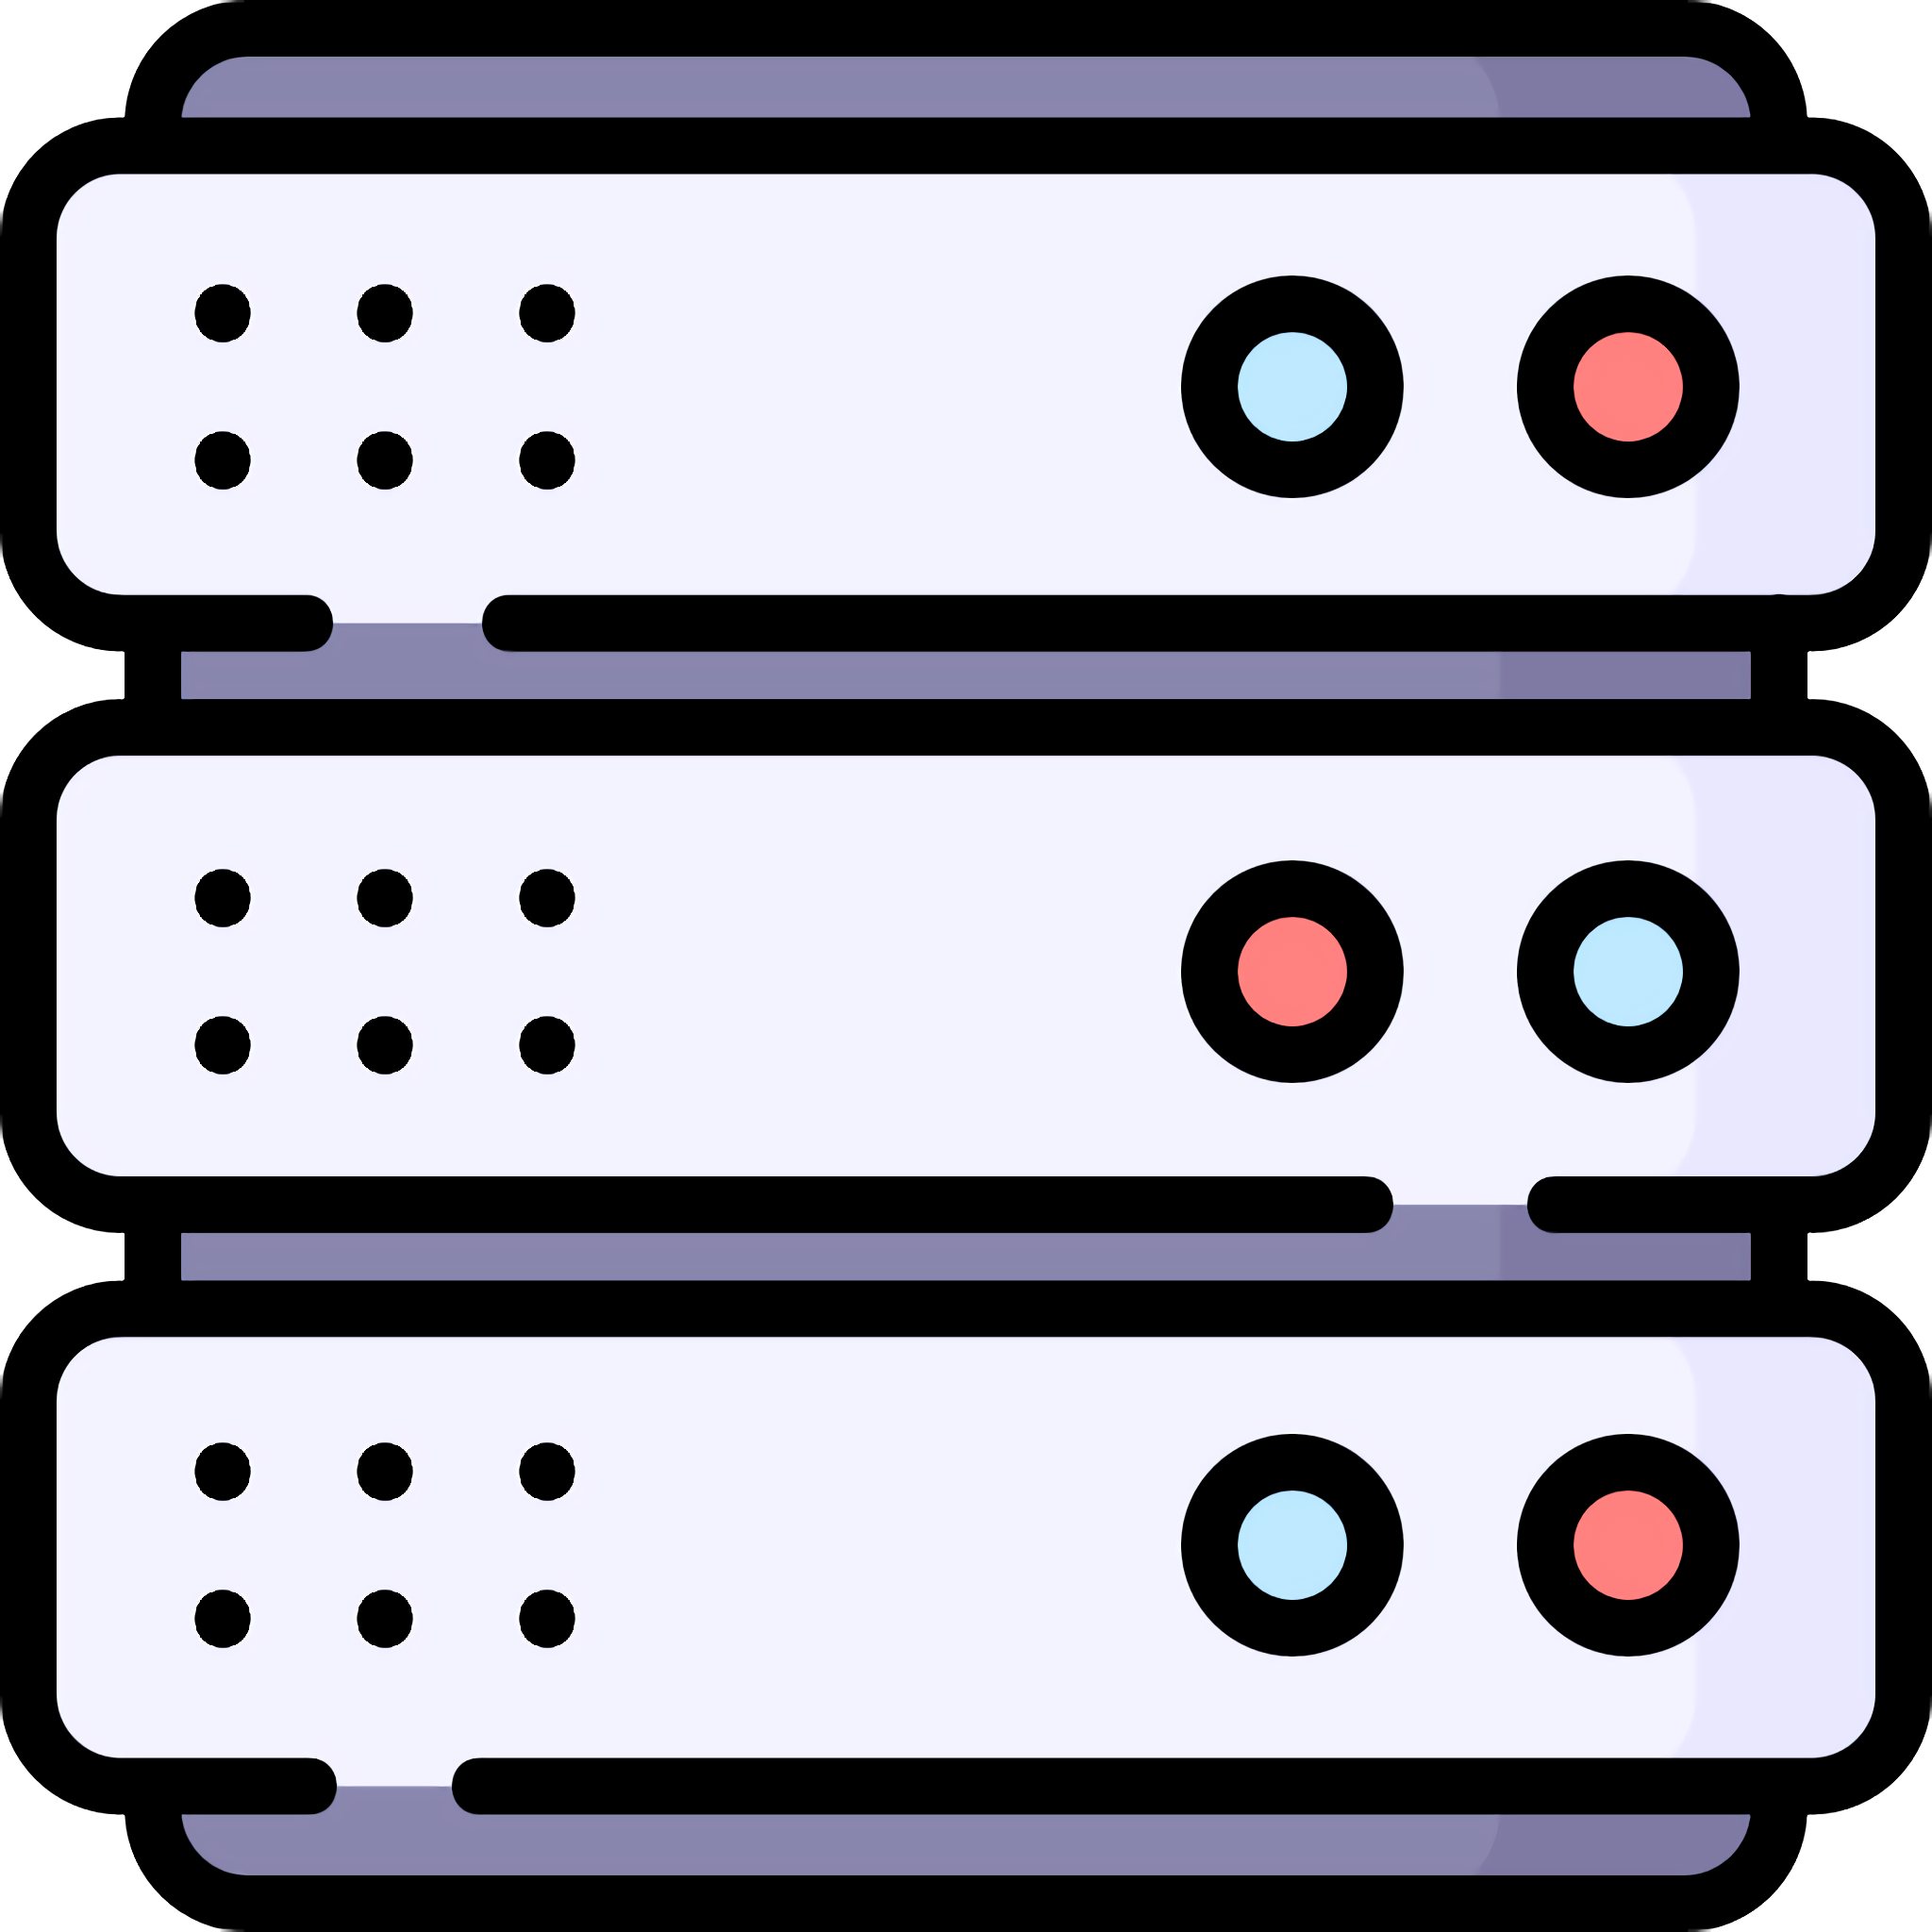
\includegraphics[scale=0.07]{images/server.png}};
    
    \draw (5) -- (6);
    \draw[rounded corners] ($(7.north west) - (0, 0.15)$) -| ++(-0.3, -0.268) |- ($(7.south west) + (0, 0.15)$);
    \draw[rounded corners] (7.east) -| ++(1,0) |- (9.west);
    \draw (9) -- (10);
    \draw (11) -- (12);
 \end{tikzpicture}
    }
\end{figure}
\end{itemize}
\end{frame}

%Normal Slide (copy, paste and modify this slide for longer presentations)
\begin{frame}
\frametitle{\secname} %Title
\framesubtitle{Topología} %Subtitle
\rmfamily %Font
\color{black} %Color
\begin{itemize}
    \item \rojoUMU{Topología} de la red.
\begin{figure}
    \centering
    \resizebox{0.8\textwidth}{!}{
        \begin{tikzpicture}
    \node (1) {
\includegraphics{cisco_icons/cloud}};
    \node (2) [below = of 1] {
\includegraphics{cisco_icons/router}};
    \node (3) [below = of 2] {$\substack{
\includegraphics{cisco_icons/pc} \\ \text{Observador}}$};
    \node (aux) [below =0.4cm of 3] {};
    \node (4) [below = of aux] {$\substack{
\includegraphics{cisco_icons/pc} \\ \text{Disp. 3}}$};
    \node (5) [left = of 4] {$\substack{
\includegraphics{cisco_icons/pc} \\ \text{Disp. 2}}$};
    \node (6) [left = of 5] {$\substack{
\includegraphics{cisco_icons/pc} \\ \text{Disp. 1}}$};
    \node (7) [right = of 4] {$\substack{
\includegraphics{cisco_icons/pc} \\ \text{Disp. 4}}$};
    \node (8) [right = of 7] {$\substack{
\includegraphics{cisco_icons/pc} \\ \text{Disp. 5}}$};
    \node (text) {Internet};
    \draw[-] (1) -- (2); 
    \draw[-] (2) -- (3);
    \draw[-] (3) -- (4);
    \draw[-] (aux.center) -| (6);
    \draw[-] (aux.center) -| (5);
    \draw[-] (aux.center) -| (7);
    \draw[-] (aux.center) -| (8);
\end{tikzpicture}
    }
\end{figure}
\end{itemize}
\end{frame}

%Normal Slide (copy, paste and modify this slide for longer presentations)
\begin{frame}
\frametitle{\secname} %Title
\framesubtitle{Recolección de datos} %Subtitle
\rmfamily %Font
\color{black} %Color
\begin{minipage}{0.5\textwidth}
\begin{itemize}
    \item La marca de tiempo relativa a cada mensaje desde el inicio, \rojoUMU{$t_i - t_{start}$}.
    \item La marca de tiempo absoluta del observador \rojoUMU{$t_i$}.
    \item La marca de tiempo absoluta del dispositivo \rojoUMU{$t'_i$}.
    \item La desviación del reloj del dispositivo respecto al del observador, \rojoUMU{$t_i - t'_i$}.
\end{itemize}
\end{minipage}
\begin{minipage}{0.3\textwidth}
\begin{figure}
    \centering
    \resizebox{1.7\textwidth}{!}{
    \begin{sequencediagram}
        \newthread{o}{Observador}
        \newinst[3]{d}{Dispositivo $x$}
        
        \begin{call}{o}{Obtener marca de tiempo}{o}{$t_i$}
        \end{call}
        
        \postlevel
        
        \begin{call}{o}{Obtener tiempo relativo al mensaje}{o}{$t_i - t_{start} \approx i$}
        \end{call}
        
        \postlevel
        
        \begin{call}{o}{Pedir marca de tiempo}{d}{Devolver $t'_i$}
        \end{call}
        
        \postlevel
        
        \begin{call}{o}{Obtener desviación}{o}{$t_i - t'_i$}
        \end{call}
    \end{sequencediagram}
    }
\end{figure}
\end{minipage}
\end{frame}

%Normal Slide (copy, paste and modify this slide for longer presentations)
\begin{frame}
\frametitle{\secname} %Title
\framesubtitle{Evaluación de los resultados} %Subtitle
\rmfamily %Font
\color{black} %Color
\begin{itemize}
    \item Evaluación de los resultados.
        \begin{itemize}
            \item Algoritmos de ML supervisados para \rojoUMU{clasificación}.
            \item Algoritmos de ML no supervisados para \rojoUMU{detección de anomalías}.
        \end{itemize}
\end{itemize}
{\small
\begin{multicols}{2}
\begin{equation*}
    Accuracy = \frac{TP + TN}{TP + FP + FN + TN}
\end{equation*}
\begin{equation*}
    Recall = \frac{TP}{TP + FN}
\end{equation*}
\begin{equation*}
    f-score = \frac{2 \cdot TP}{2 \cdot TP + FP + FN}
\end{equation*}
\begin{equation*}
    TNR = \frac{TN}{TN + FP}
\end{equation*}
\end{multicols}
}
\end{frame}







\section{Experimentos}

%Normal Slide (copy, paste and modify this slide for longer presentations)
\begin{frame}
\frametitle{\secname} %Title
\framesubtitle{Comparativa de los experimentos} %Subtitle
\rmfamily %Font
\color{black} %Color
\begin{table}
    \centering
    \resizebox{0.75\textwidth}{!}{
    \begin{tabular}{ccccc}
        \toprule
        \texttt{time} & \texttt{TSrock} & \texttt{TSrasp} & \texttt{offset} & \texttt{device} \\
        \midrule
        292 & 119238112796030 & 104592709716803 & -14645403079227 & 192.168.1.111 \\
        1001191222 & 119239113986960 & 104593710167425 & -14645403819535 & 192.168.1.111 \\
        2001485862 & 119240114281600 & 104594710453699 & -14645403827901 & 192.168.1.111 \\
        \vdots & \vdots & \vdots & \vdots & \vdots \\
        \bottomrule
    \end{tabular}
    }
    \caption{Ejemplo de los datos obtenidos de cada dispositivo}
    \label{tab:trace_example}
\end{table}
\vspace{-1.3cm}
\setcounter{subfigure}{0}
\begin{figure}
    \centering
    \subfloat[Desviación acumulada muestra secuencial]{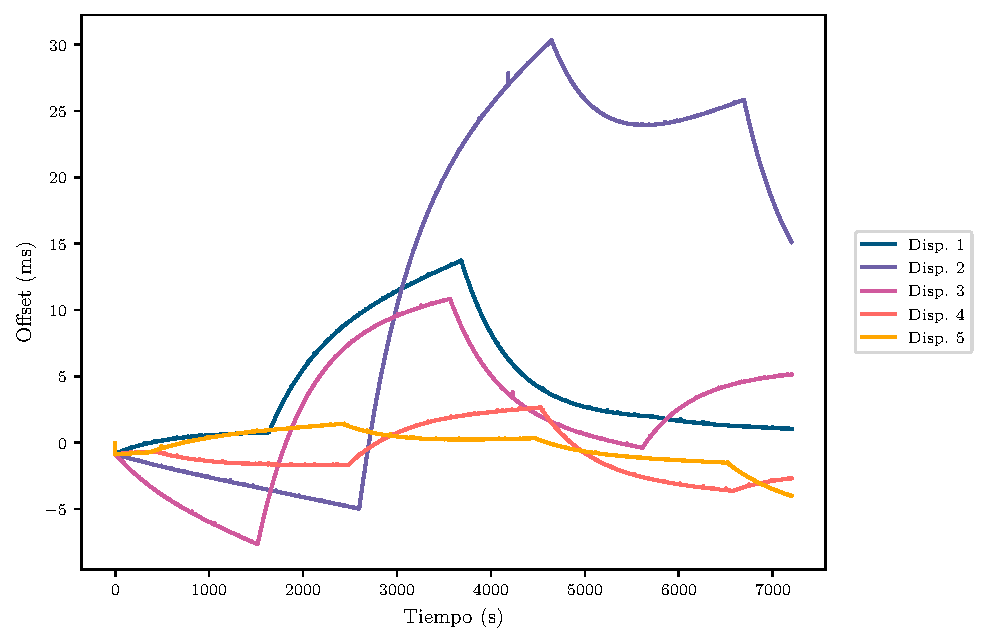
\includegraphics[width=0.5\textwidth]{../Python/plots/individual/offset_plot.pdf}}
    \subfloat[Desviación acumulada muestra paralela]{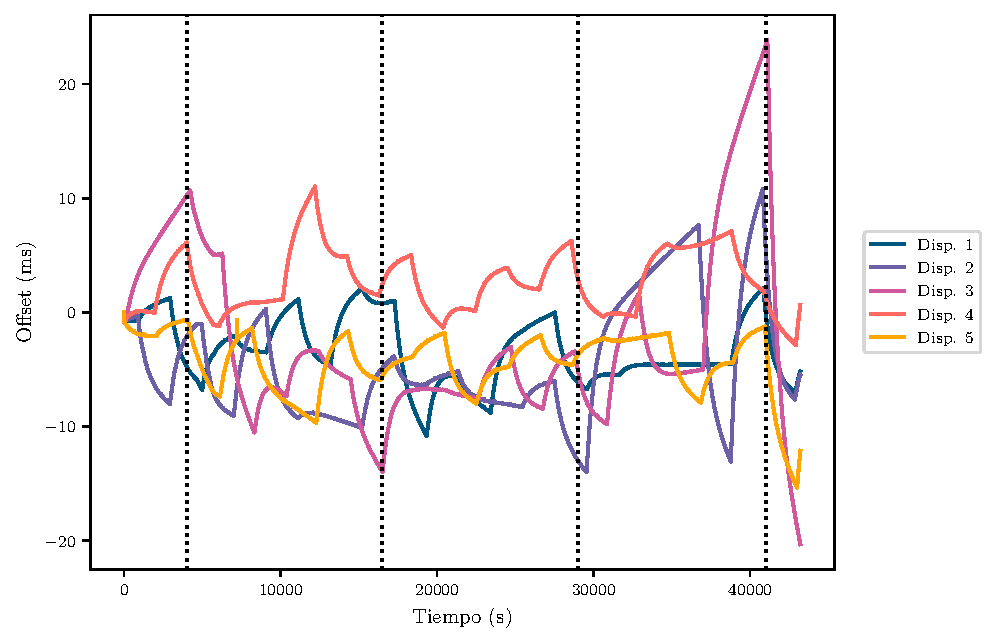
\includegraphics[width=0.5\textwidth]{../Python/plots/parallel/offset_plot.pdf}}
\end{figure}
\end{frame}

%Normal Slide (copy, paste and modify this slide for longer presentations)
\begin{frame}
\frametitle{\secname} %Title
\framesubtitle{Comparativa de los experimentos} %Subtitle
\rmfamily %Font
\color{black} %Color
\setcounter{subfigure}{0}
\begin{figure}
    \centering
    \subfloat[Desviación muestra secuencial]{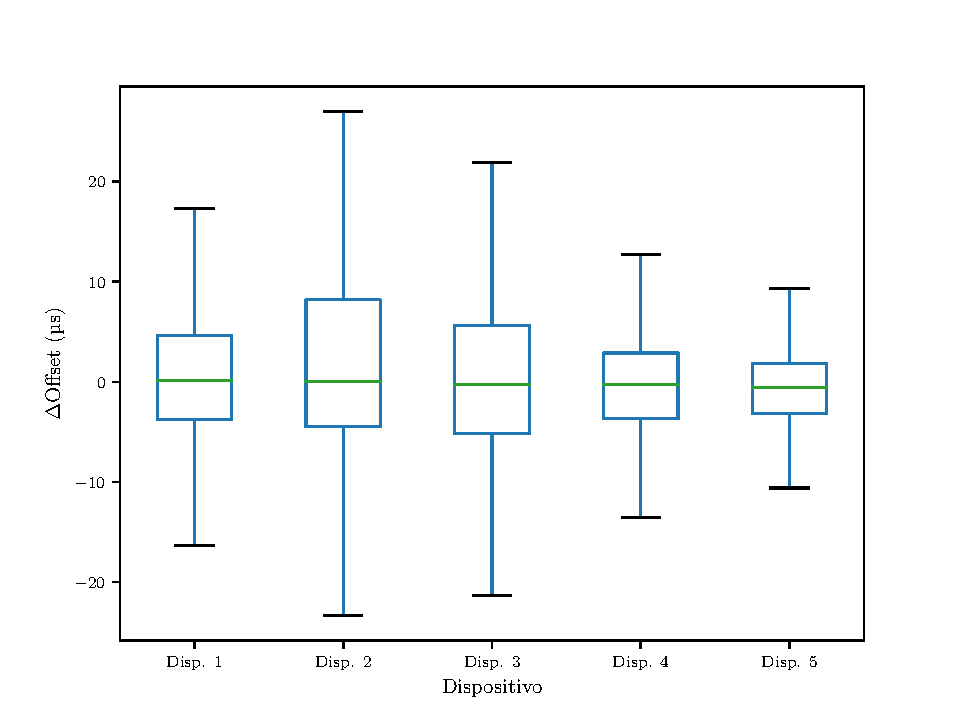
\includegraphics[width=0.5\textwidth]{../Python/plots/individual/boxplot_no_out.pdf}}
    \subfloat[Desviación muestra paralela]{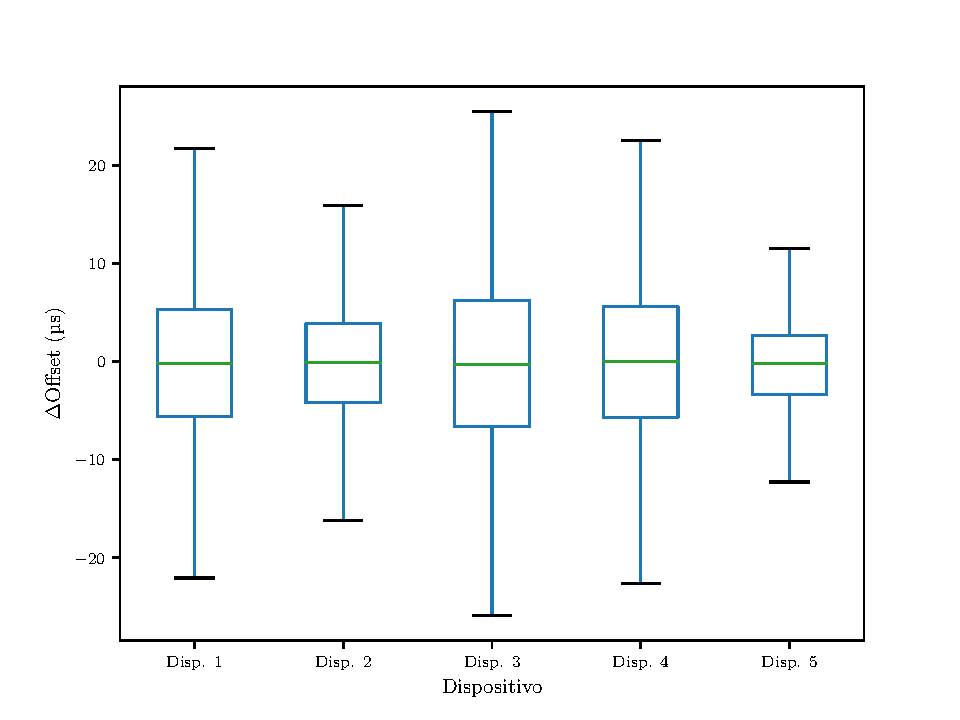
\includegraphics[width=0.5\textwidth]{../Python/plots/parallel/boxplot_no_out.pdf}}
\end{figure}
\end{frame}

%Normal Slide (copy, paste and modify this slide for longer presentations)
\begin{frame}
\frametitle{\secname} %Title
\framesubtitle{Generación de estadísticas y reducción de la \\[-2pt] dimensionalidad} %Subtitle
\rmfamily %Font
\color{black} %Color
\begin{table}
    \centering
    \resizebox{\textwidth}{!}{
        \begin{tabular}{cccccccccccc}
            \toprule
             & Sum & Mean & Median & Mode & Std & IQR & Kurtosis & Skew & Max & Min & Device \\
            \midrule
            1 & -284.0 & -4.733333333333333 & -203.0 & -10750.0 & 6531.321744049499 & 8739.5 & -0.8026364427898236 & 0.266444555013173 & 12077.0 & -10750.0 & Disp. 1 \\
            2 & -65895.0 & -1098.25 & 106.5 & -13344.0 & 3926.559099283938 & 2519.75 & 1.4605213340303709 & -1.1040127142547507 & 7616.0 & -13344.0 & Disp. 2 \\
            3 & 96179.0 & 1602.9833333333333 & 815.0 & -8136.0 & 5010.092595279735 & 6575.5 & -0.39715065367509084 & 0.2484646585713819 & 12831.0 & -8136.0 & Disp. 3 \\
            4 & 109162.0 & 1819.3666666666666 & 2016.5 & -10485.0 & 6159.084454763058 & 8290.5 & -0.7264084617343212 & -0.3858981208999922 & 11469.0 & -10485.0 & Disp. 4 \\
            5 & -81317.0 & -1355.2833333333333 & -2127.0 & -6378.0 & 3665.051390911538 & 2616.5 & 2.701193448053943 & 1.7089231615691112 & 10383.0 & -6378.0 & Disp. 5 \\
            6 & 19928.0 & 332.1333333333333 & -147.0 & -10750.0 & 6613.483928825726 & 10212.0 &     -0.8404647945245984 & 0.23473423365399895 & 12077.0 & -10750.0 & Disp. 1 \\
            \vdots & \vdots & \vdots & \vdots & \vdots & \vdots & \vdots & \vdots & \vdots & \vdots & \vdots & \vdots \\
            \bottomrule
        \end{tabular}
    }
    \caption{Datos estadísticos muestra paralela}
    \label{tab:stats_par}
\end{table}
\vspace{-1cm}
\begin{figure}
    \centering
    \subfloat{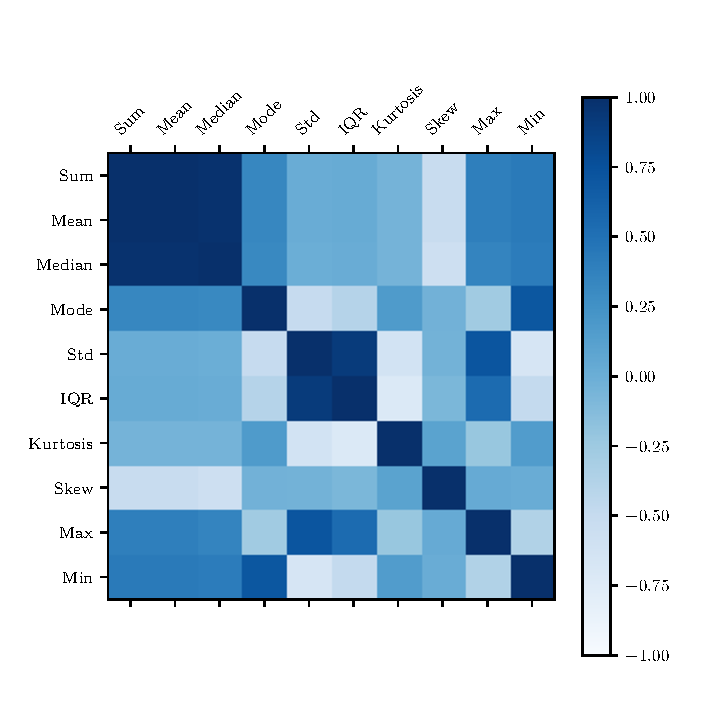
\includegraphics[scale=0.3]{../Python/plots/parallel/correlacion_stats.pdf}}
    \subfloat{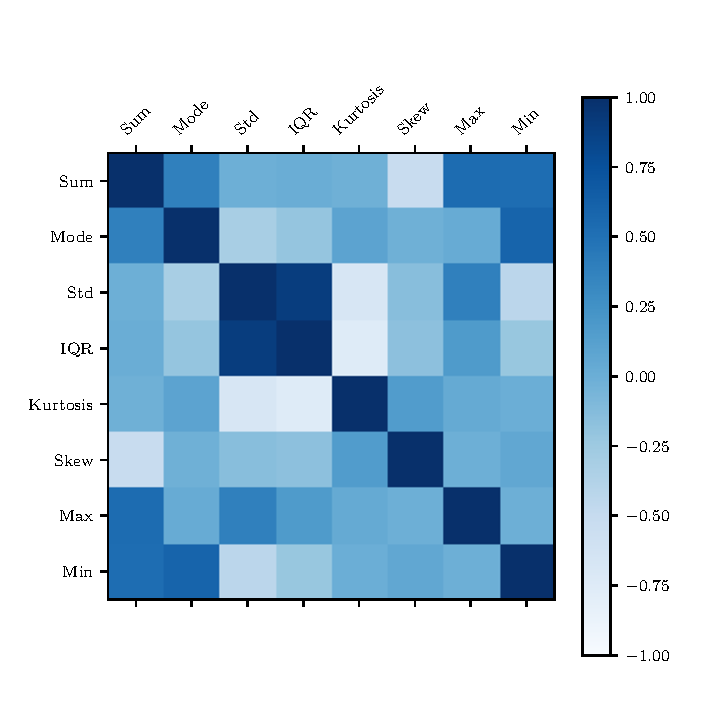
\includegraphics[scale=0.3]{../Python/plots/parallel/correlacion_stats_ftred.pdf}}
    \caption{Correlación entre las variables estadísticas}
    \label{fig:corr}
\end{figure} 
\end{frame}

%Normal Slide (copy, paste and modify this slide for longer presentations)
\begin{frame}
\frametitle{\secname} %Title
\framesubtitle{Particionamiento de los datos} %Subtitle
\rmfamily %Font
\color{black} %Color
\begin{figure}
    \centering
    \hspace{-0.65cm}
    \subfloat[Particionamiento para clasificadores]{
        \resizebox{0.6\textwidth}{!}{
            \begin{tikzpicture}[show background rectangle,background rectangle/.style={fill=white, draw, rounded corners, thick}]
                \node[database,label=below:Datos del dispositivo,database radius=1cm,database segment height=0.5cm] (data) {};
                \node (aux) [right = of data] {};
                \node[database,label=below:Entrenamiento,database radius=0.75cm,database segment height=0.375cm] (train) [above right = 2cm of aux] {};
                \node[database,label=below:Test,database radius=0.75cm,database segment height=0.375cm] (test) [below right = 2cm of aux] {};
                \node[database,label=below:{$\underset{\text{Reducido}}{\text{Entrenamiento}}$},database radius=0.5cm,database segment height=0.25cm] (train2) [right = 3cm of train] {};
                \node (aux2) [right = of train2] {};
                \node[database,label=below:Entrenamiento,label=right:70\%,database radius=0.5cm,database segment height=0.25cm] (train3) [above right = of aux2] {};
                \node[database,label=below:Validación,label=right:30\%,database radius=0.5cm,database segment height=0.25cm] (test) [below right = of aux2] {};
                \draw[-] (1.2,0) -- (aux.center);
                \draw[-] (aux.center) |- (3.4, 2.4) node [above, pos=0.75] {70\%};
                \draw[-] (aux.center) |- (3.4, -2.45) node [below, pos=0.75] {30\%};
                \draw[-] (5.5, 2.4) -- (8, 2.4) node [midway, above] {35\%};
                \draw[-] (9.5, 2.4) -- (aux2.center);
                \draw[-] (aux2.center) |- (11.3, 4.1);
                \draw[-] (aux2.center) |- (11.3, 0.66);
            \end{tikzpicture}
        }
    }
    \subfloat[Particionamiento para la detección de anomalías]{
        \resizebox{0.4\textwidth}{!}{
            \begin{tikzpicture}[show background rectangle,background rectangle/.style={fill=white, draw, rounded corners, thick}]
                \node[database,label=below:Datos,database radius=1cm,database segment height=0.5cm, outer sep=0.5cm] (data) {};
                \node[database,label=below:$\underset{\text{Disp. }x}{\text{Datos}}$,database radius=0.75cm,database segment height=0.375cm, outer sep=0.3cm] (disp_data) [above right = 0cm and 2cm of data] {};
                \node[database,label=below:$\underset{\text{sin Disp. }x}{\text{Datos}}$,database radius=0.75cm,database segment height=0.375cm, outer sep=0.3cm] (disp_out_data) [below right = 0cm and 2cm of data] {};
                
                \node[database,label=below:Entrenamiento,database radius=0.75cm,database segment height=0.375cm, outer sep=0.3cm] (train) [above right = -0.5cm and 2cm of disp_data] {};
                \node[database,label=below:Test,database radius=0.75cm,database segment height=0.375cm, outer sep=0.3cm] (test) [below right = -1cm and 2cm of disp_data] {};
                
                
                \node (train2) [above right = -1cm and 2cm of disp_out_data] {\Huge\phantom{---}\xmark};
                \node[database,label=below:Test,database radius=0.75cm,database segment height=0.375cm, outer sep=0.3cm] (test2) [below right = -1cm and 2cm of disp_out_data] {};
                
                \draw[-] (data) -| (2.4,0) |- (disp_data);
                \draw[-] (data) -| (2.4,0) |- (disp_out_data);
                
                \draw[-] (disp_data) -| (6.4, 4) |- (train) node [above, pos=0.75] {80\%};
                \draw[-] (disp_data) -| (6.4, 4) |- (test) node [above, pos=0.75] {20\%};
                
                \draw[-] (disp_out_data) -| (6.4, -4) |- (train2) node [above, pos=0.75] {80\%};
                \draw[-] (disp_out_data) -| (6.4, -4) |- (test2) node [above, pos=0.75] {20\%};
                
            \end{tikzpicture}
        }
    }
\end{figure}
\end{frame}

\section{Resultados}

%Normal Slide (copy, paste and modify this slide for longer presentations)
\begin{frame}
\frametitle{\secname} %Title
\framesubtitle{Comparativa de algoritmos} %Subtitle
\rmfamily %Font
\color{black} %Color
\begin{figure}
    \centering
    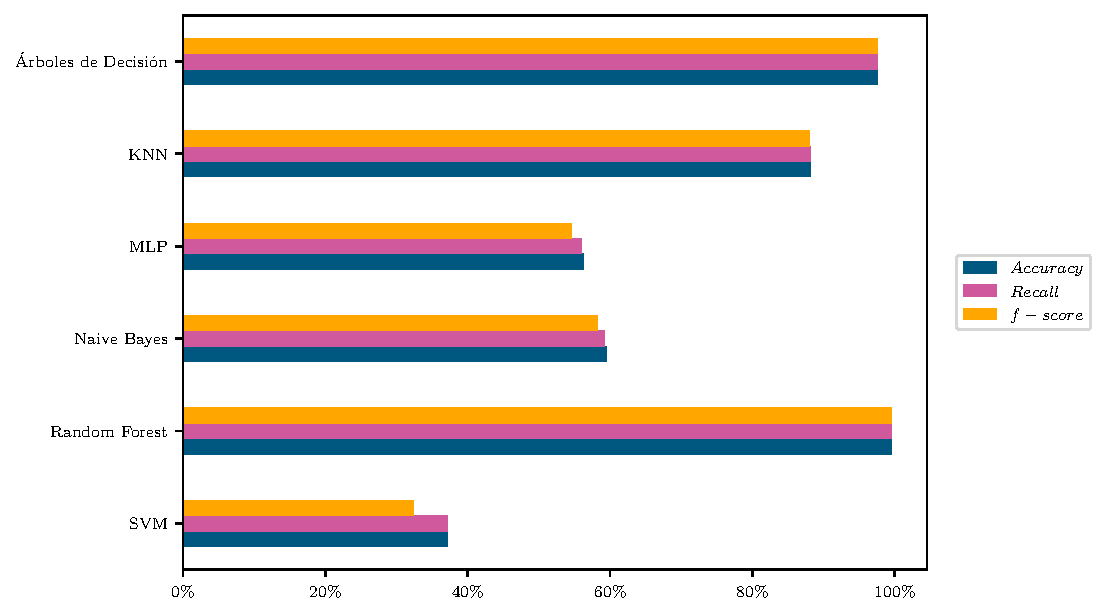
\includegraphics[width=0.6\textwidth]{../Python/plots/parallel/model_results.pdf}
    \caption{Algoritmos de clasificación}
\end{figure} 
\vspace{-1cm}
\begin{table}
    \centering
    \resizebox{0.5\textwidth}{!}{
        \begin{tabular}{lcccccc}
    \toprule
     & \multicolumn{2}{c}{\texttt{Isolation Forest}} & \multicolumn{2}{c}{\texttt{Local Outlier Factor}} & \multicolumn{2}{c}{\texttt{OneClass-SVM}} \\
    \cmidrule(lr){2-3}\cmidrule(lr){4-5}\cmidrule(lr){6-7}
    & $Recall$ & $TNR$ & $Recall$ & $TNR$ & $Recall$ & $TNR$ \\
    \midrule
     Disp. 1 & 95.12\% & 10.36\% & 98.99\% & 10.68\% & 49.48\% & 58.24\% \\
     Disp. 2 & 94.98\% & 28.87\% & 98.45\% & 57.74\% & 50.90\% & 70.36\% \\
     Disp. 3 & 94.80\% & 13.90\% & 98.73\% & 13.64\% & 49.84\% & 52.65\% \\
     Disp. 4 & 95.80\% & 16.61\% & 98.88\% & 8.74\% & 50.54\% & 64.66\% \\
     Disp. 5 & 94.89\% & 46.99\% & 98.63\% & 77.98\% & 49.53\% & 94.59\% \\
    \bottomrule
\end{tabular}

    }
    \caption{Algoritmos de detección de anomalías}
\end{table}
\end{frame}


%Normal Slide (copy, paste and modify this slide for longer presentations)
\begin{frame}
\frametitle{\secname} %Title
\framesubtitle{Resultados finales} %Subtitle
\rmfamily %Font
\color{black} %Color
\begin{minipage}{0.4\textwidth}
Resultados:
    \begin{itemize}
        \item Accuracy: 99.38\%
        \item $f$-score: 99.38\%
        \item Recall: 99.39\%
    \end{itemize}
\end{minipage}
\begin{minipage}{0.43\textwidth}
\begin{figure}
    \centering
    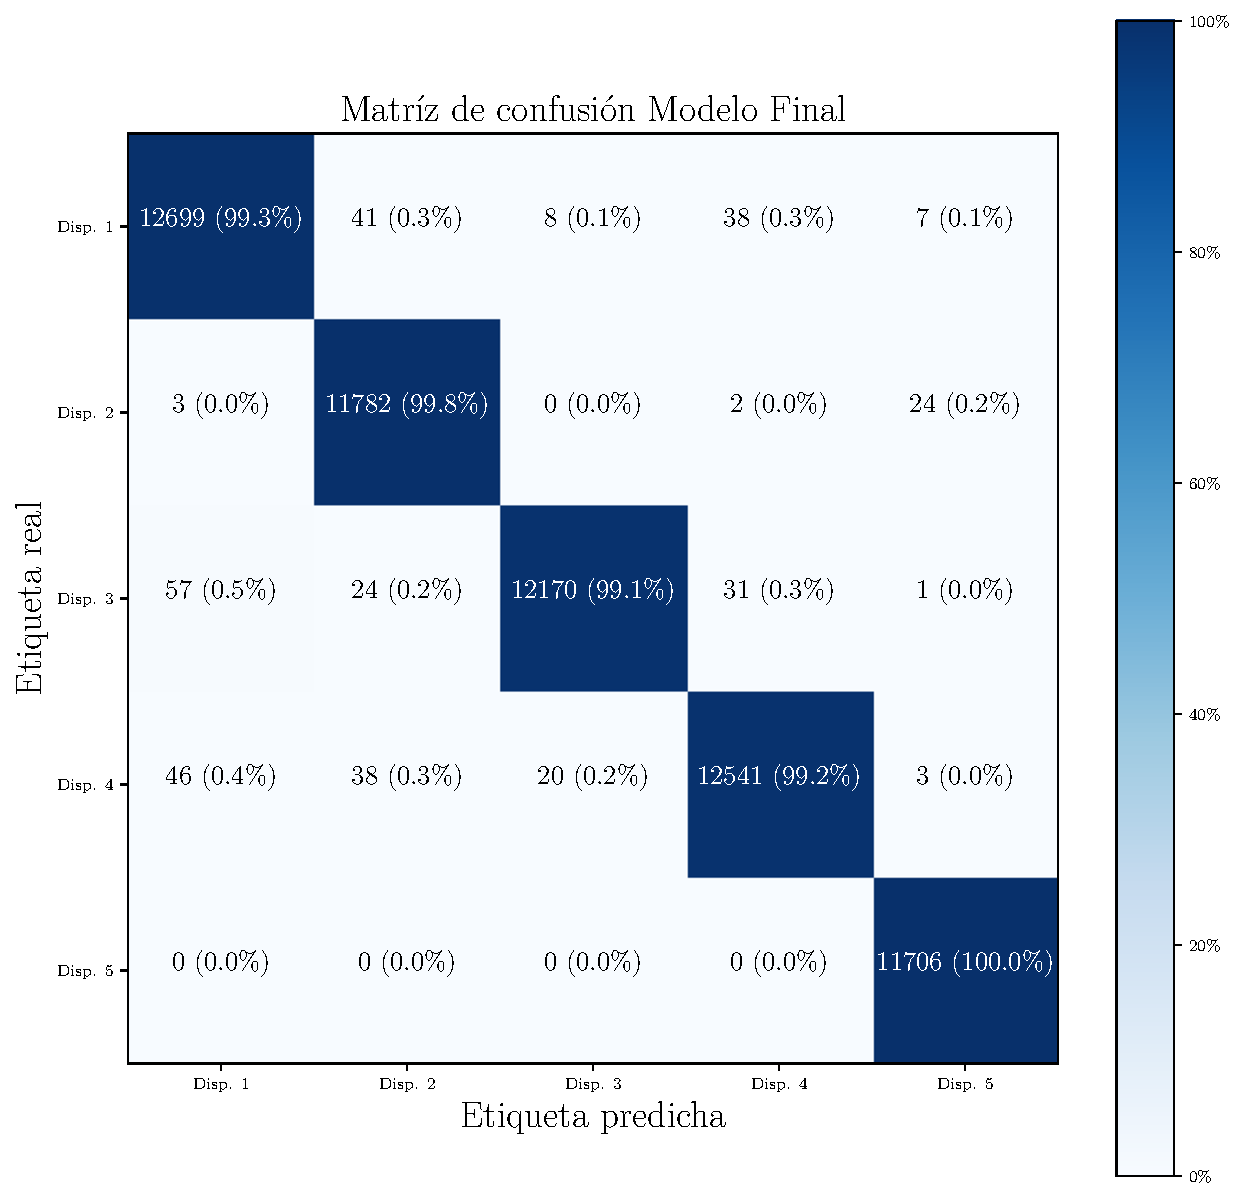
\includegraphics[width=1.6\textwidth]{../Python/plots/parallel/final_model_matrix.pdf}
\end{figure}
\end{minipage}
\end{frame}



%!TEX root = TFG.tex

\chapter{Conclusiones y vías futuras} \label{chap:conclu}

En este proyecto hemos diseñado un modelo capaz de clasificar dispositivos con los que nos estamos comunicando en base a pequeñas diferencias en la fabricación de los componentes, que altera el tiempo que tardan en ejecutar una cierta tarea.

En la primera parte del proyecto hemos visto como para obtener la precisión en los tiempos que queríamos hemos tenido que usar el protocolo TCP y enviar las marcas de tiempo en el cuerpo del paquete. 

En este momento se vio que el interno es susceptible de ser alterado por procesos externos para que esté sincronizado en todo momento con el resto de los dispositivos (protocolo NTP), por este motivó este servicio tuvo que ser desactivado antes de realizar ninguna captura de paquetes, pues los diferencias entre tiempos no serían las propias del dispositivo.

Una vez desactivado el servicio, aún se obtenían datos que no eran correctos debido a que se estaba usando un reloj del sistema que podía ser modificado. Este reloj fue cambiado por un reloj que no fuera modificable (\texttt{steady\_clock}) y con eso los datos fueron más precisos.

Se realizaron capturas tanto en secuencial como en paralelo de la desviación de los relojes de los dispositivos, de las cuales se obtuvieron sus incrementos en cada momento. Con estos incrementos y una ventana deslizante de 1 minuto se obtienen variables estadísticas que servirán para entrenar los modelos.

Después de ver los resultados de los modelos con los conjuntos de entrenamiento/validación y analizando los posibles usos del sistema implementado se considera que es mejor quedarse con la muestra paralela. 

Por último entrenamos el modelo elegido, Random Forest, con los datos de la muestra paralela y los hiperparámetros que se consideraron mejores cuando se realizó el entrenamiento los conjuntos de entrenamiento/validación. De este modelo obtenemos unos resultados finales de 99.44\% en el valor de accuracy.

Como posibles vías futuras de este trabajo estaría el desarrollo de un modelo a tiempo real de este sistema. Para este cometido se debería tener una copia local de las huellas que generan ciertos dispositivos para poder compararlos con los que estamos recibiendo en ese momento y así comprobar si se trata de un atacante.

Para realizar este sistema a tiempo real también habría que crear mecanismos que permitan al sistema actualizarse con nuevos datos, y con ello generar nuevas huellas para los dispositivos. También habría que modificar los modelos de machine learning debido a que para que el sistema funcione a tiempo real, estos deberían actualizarse. 




% Questions slide
{\usebackgroundtemplate{\includegraphics[width=\paperwidth]{/Users/serms1999/Pictures/Fondo2.png}} %Contents Background
\begin{frame}
\frametitle{} %Contents Title
\rmfamily %Contents Font
\color{white}
\Large\bfseries
\vfill\vspace{3cm}
Gracias por su atención. \\
¿Alguna pregunta? \\
\sigField{Firma}{5cm}{3cm} \\
\vfill

\end{frame}
}

\end{document}
